
\documentclass[10pt]{article}
 
\usepackage[T1]{fontenc}
\usepackage[utf8]{inputenc}
\usepackage{microtype}
\usepackage{XCharter}
\usepackage{amsmath, amssymb}
 
\usepackage[
  paperwidth=8.5in, paperheight=11in,
  margin=0.6in
]{geometry}
 
\usepackage[dvipsnames]{xcolor}
\definecolor{deepblue}{RGB}{20, 50, 100}
\definecolor{lightblue}{RGB}{190,210,245}
\definecolor{warmgold}{RGB}{170,130,40}
\definecolor{softgreen}{RGB}{50,130,70}
\definecolor{manifoldcolor}{RGB}{232,240,255}
\definecolor{distcolor}{RGB}{235,248,238}
\definecolor{midblue}{RGB}{60,100,170}
 
\usepackage{tikz}
\usetikzlibrary{arrows.meta, calc, positioning,
  decorations.pathmorphing, decorations.markings,
  shapes.geometric, patterns}
 
\tikzset{
  >=Stealth,
  mapsto/.style={->, line width=1.3pt, deepblue},
  pullbackarrow/.style={->, line width=1.2pt, warmgold},
  dfstyle/.style={->, line width=0.9pt, midblue, dashed},
  tanvec/.style={->, line width=1.5pt},
  mbox/.style={fill=manifoldcolor, draw=deepblue!40,
               line width=0.8pt, rounded corners=5pt, inner sep=8pt},
  pbox/.style={fill=distcolor, draw=softgreen!50,
               line width=0.8pt, rounded corners=5pt, inner sep=8pt},
}
 
\usepackage{caption}
\captionsetup{font=small, labelfont=bf, width=0.92\linewidth}
\usepackage{parskip}
\setlength{\parindent}{0pt}
 
\begin{document}
 
\section*{Chapter 1 --- Figure 1: Pullback origin of the FIM}
 
% --- Figure 1: Pullback construction ---
\begin{figure}[h]
\centering
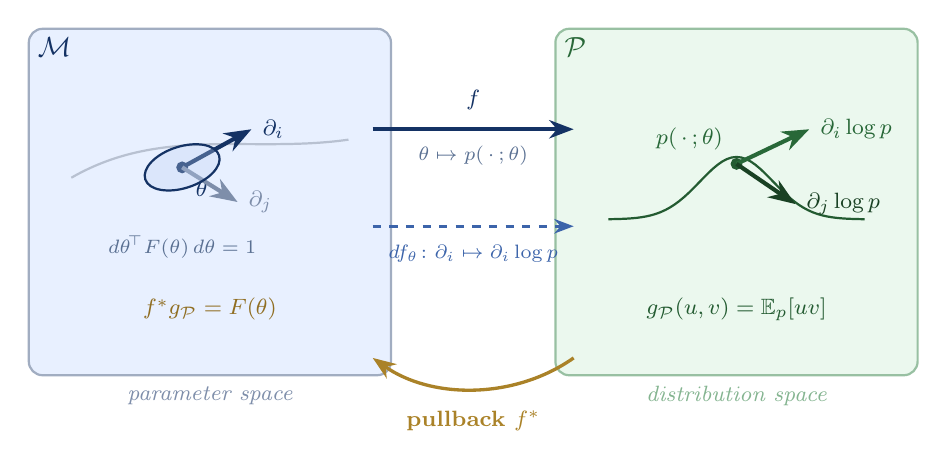
\begin{tikzpicture}[font=\small, scale=0.88]
 
  % ---- Left box M ----
  \node[mbox, minimum width=4.6cm, minimum height=4.4cm]
    (Mbox) at (0,0) {};
  \node[anchor=north west, deepblue, font=\normalsize\bfseries,
        inner sep=0] at ($(Mbox.north west)+(0.14,-0.14)$)
    {$\mathcal{M}$};
  \node[deepblue!55, font=\footnotesize\itshape]
    at ($(Mbox.south)+(0,-0.28)$) {parameter space};
 
  \draw[deepblue!30, thick]
    (-2.0, 0.35) .. controls (-0.7,1.1) and (0.6,0.7) .. (2.0, 0.9);
 
  \coordinate (th) at (-0.4, 0.5);
  \filldraw[deepblue] (th) circle (2.2pt);
  \node[deepblue, below right=2pt, font=\footnotesize] at (th)
    {$\theta$};
 
  \draw[tanvec, deepblue]    (th) -- ++(1.0, 0.55)
    node[right, font=\footnotesize] {$\partial_i$};
  \draw[tanvec, deepblue!55] (th) -- ++(0.8,-0.50)
    node[right, font=\footnotesize] {$\partial_j$};
 
  \draw[deepblue, thick, fill=lightblue, fill opacity=0.3,
        rotate around={18:(th)}] (th) ellipse (0.56cm and 0.30cm);
 
  \node[deepblue!70, font=\scriptsize] at (-0.4,-0.65)
    {$d\theta^{\!\top}F(\theta)\,d\theta=1$};
 
  \node[warmgold!85!black, font=\footnotesize\bfseries]
    at (0,-1.55) {$f^*g_{\mathcal{P}}=F(\theta)$};
 
  % ---- Right box P ----
  \node[pbox, minimum width=4.6cm, minimum height=4.4cm]
    (Pbox) at (7.6,0) {};
  \node[anchor=north west, softgreen!80!black,
        font=\normalsize\bfseries, inner sep=0]
    at ($(Pbox.north west)+(0.14,-0.14)$) {$\mathcal{P}$};
  \node[softgreen!60, font=\footnotesize\itshape]
    at ($(Pbox.south)+(0,-0.28)$) {distribution space};
 
  \begin{scope}[shift={(7.6,0)}]
    \coordinate (pfth) at (0.0, 0.55);
    \draw[softgreen!70!black, thick, domain=-1.85:1.85, samples=55]
      plot (\x, {0.90*exp(-1.8*\x*\x) - 0.25});
    \filldraw[softgreen!70!black] (pfth) circle (2.2pt);
    \node[softgreen!80!black, above left=2pt, font=\footnotesize]
      at (pfth) {$p(\,\cdot\,;\theta)$};
 
    \draw[tanvec, softgreen!80!black]
      (pfth) -- ++(1.05, 0.50)
      node[right, font=\footnotesize] {$\partial_i\log p$};
    \draw[tanvec, softgreen!50!black]
      (pfth) -- ++(0.85,-0.58)
      node[right, font=\footnotesize] {$\partial_j\log p$};
 
    \node[softgreen!70!black, font=\footnotesize\bfseries]
      at (0.0,-1.55) {$g_{\mathcal{P}}(u,v)=\mathbb{E}_p[uv]$};
  \end{scope}
 
  % ---- Map arrow f (above centre) ----
  \draw[mapsto]
    (2.35, 1.05) -- (5.25, 1.05)
    node[midway, above=3pt, font=\footnotesize\bfseries, deepblue]
      {$f$}
    node[midway, below=2pt, font=\scriptsize, deepblue!70]
      {$\theta\mapsto p(\,\cdot\,;\theta)$};
 
  % ---- Differential df (below centre) ----
  \draw[dfstyle]
    (2.35,-0.35) -- (5.25,-0.35)
    node[midway, below=3pt, font=\scriptsize, midblue]
      {$df_\theta\colon\partial_i\mapsto\partial_i\log p$};
 
  % ---- Pullback arc (below both boxes) ----
  \draw[pullbackarrow]
    (5.25,-2.25)
    .. controls (4.4,-2.85) and (3.2,-2.85) ..
    (2.35,-2.25)
    node[midway, below=4pt, font=\footnotesize\bfseries, warmgold]
      {pullback $f^*$};
 
\end{tikzpicture}
\caption{The pullback origin of the Fisher Information Matrix.
  The Fisher metric is inherited from $\mathcal{P}$ through $f$.
  The differential $df_\theta$ pushes tangent vectors forward;
  the $L^2$ inner product on score functions pulls back to give
  $F_{ij}(\theta)=\mathbb{E}_\theta[\partial_i\log p
  \cdot\partial_j\log p]$.}
\end{figure}
 
\clearpage
\section*{Chapter 1 --- Figure 2: Fisher ellipses and Cram\'{e}r--Rao}
 
% --- Figure 2: Statistical manifold with Fisher ellipses ---
\begin{figure}[h]
\centering
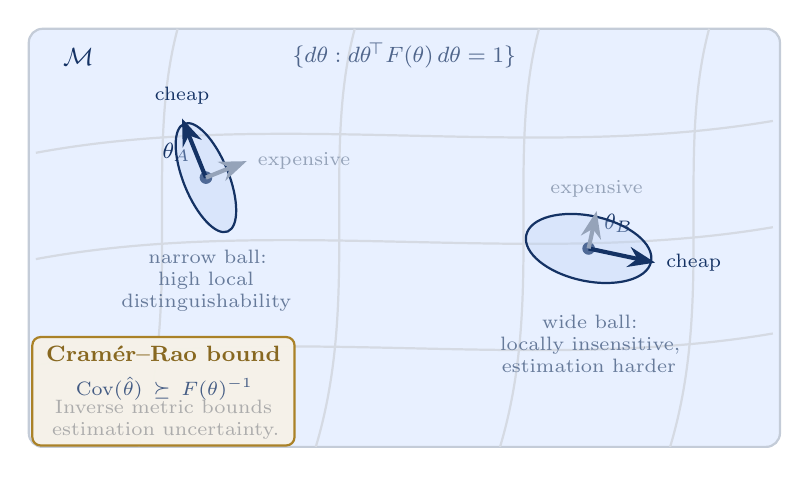
\begin{tikzpicture}[font=\small, scale=0.90]
  \fill[manifoldcolor, rounded corners=5pt]
    (-5.3,-3.1) rectangle (5.3,2.8);
  \draw[deepblue!25, rounded corners=5pt, thick]
    (-5.3,-3.1) rectangle (5.3,2.8);
  \foreach \ya in {-1.7,-0.2,1.3}{
    \draw[deepblue!18,thick]
      (-5.2,\ya-0.25) .. controls (-1.8,\ya+0.38)
                      and (1.8,\ya-0.38) .. (5.2,\ya+0.2);
  }
  \foreach \xa in {-3.4,-0.9,1.7,4.1}{
    \draw[deepblue!18,thick]
      (\xa-0.35,-3.1) .. controls (\xa+0.28,-1.0)
                      and (\xa-0.28,1.0) .. (\xa+0.2,2.8);
  }
  \node[deepblue,font=\small\bfseries] at (-4.6,2.4) {$\mathcal{M}$};
 
  % Point A: narrow ellipse
  \coordinate (ptA) at (-2.8, 0.7);
  \filldraw[deepblue] (ptA) circle (2.3pt);
  \node[deepblue,above left=3pt,font=\footnotesize\bfseries]
    at (ptA) {$\theta_A$};
  \draw[deepblue,thick,fill=lightblue,fill opacity=0.35,
        rotate around={22:(ptA)}]
    (ptA) ellipse (0.32cm and 0.82cm);
  \draw[tanvec,deepblue,rotate around={22:(ptA)}]
    (ptA) -- ++(0, 0.90)
    node[above,font=\scriptsize,yshift=1pt] {cheap};
  \draw[tanvec,deepblue!45,rotate around={22:(ptA)}]
    (ptA) -- ++(0.62, 0)
    node[right,font=\scriptsize] {expensive};
  \node[deepblue!65,font=\scriptsize,align=center,text width=2.5cm]
    at (-2.8,-0.75)
    {narrow ball:\\high local\\distinguishability};
 
  % Point B: wide ellipse
  \coordinate (ptB) at (2.6,-0.3);
  \filldraw[deepblue] (ptB) circle (2.3pt);
  \node[deepblue,above right=3pt,font=\footnotesize\bfseries]
    at (ptB) {$\theta_B$};
  \draw[deepblue,thick,fill=lightblue,fill opacity=0.35,
        rotate around={-12:(ptB)}]
    (ptB) ellipse (0.90cm and 0.46cm);
  % "cheap" now correctly along the LONG axis (0.90cm)
  \draw[tanvec,deepblue,rotate around={-12:(ptB)}]
    (ptB) -- ++(0.96, 0)
    node[right,font=\scriptsize] {cheap};
  % "expensive" now correctly along the SHORT axis (0.46cm)
  \draw[tanvec,deepblue!45,rotate around={-12:(ptB)}]
    (ptB) -- ++(0, 0.54)
    node[above,font=\scriptsize,yshift=1pt] {expensive};
  \node[deepblue!65,font=\scriptsize,align=center,text width=2.5cm]
    at (2.6,-1.65)
    {wide ball:\\locally insensitive,\\estimation harder};
 
  % Unit ball label
  \node[deepblue!75,font=\footnotesize,align=center]
    at (0, 2.42)
    {$\{d\theta:d\theta^{\!\top}F(\theta)\,d\theta=1\}$};
 
  % Cramer-Rao inset — left side
  \draw[warmgold,thick,rounded corners=3pt,
        fill=warmgold!10,fill opacity=0.97]
    (-5.25,-3.08) rectangle (-1.55,-1.55);
  \node[warmgold!80!black,font=\footnotesize\bfseries]
    at (-3.40,-1.78) {Cram\'{e}r--Rao bound};
  \node[font=\scriptsize,align=center,text width=3.0cm,deepblue!80]
    at (-3.40,-2.28)
    {$\mathrm{Cov}(\hat\theta)\succeq F(\theta)^{-1}$};
  \node[font=\scriptsize,align=center,text width=3.0cm,gray!65]
    at (-3.40,-2.72)
    {Inverse metric bounds\\estimation uncertainty.};
 
\end{tikzpicture}
\caption{The Fisher metric as a varying Riemannian structure on
  $\mathcal{M}$. At $\theta_A$ the ellipse is narrow:
  distributions change rapidly with $\theta$, estimation is easy.
  At $\theta_B$ the ellipse is wide: distributions change slowly
  with $\theta$, so estimation is harder. The Cram\'{e}r--Rao
  bound (inset) quantifies this precisely.}
\end{figure}